\documentclass[captions=tableheading]{scrartcl}
\usepackage{microtype}
\usepackage{amsmath}
\usepackage{polyglossia}
\usepackage{graphicx}
\usepackage{booktabs}
\usepackage{siunitx}
\usepackage{hyperref}
\usepackage{caption}
\usepackage{float}

\begin{document}
    
\section{Aufgabe 7a}

Zuerst werden die Werte aus \ref{tab:7a} in einem Diagramm dargestellt.
Dazu werden auch noch Fehlerbalken dargestellt,
welche die Unsicherheit der Messwerte von $\sqrt{N}$ anzeigen.

\noindent Es sieht folgendermaßen aus:

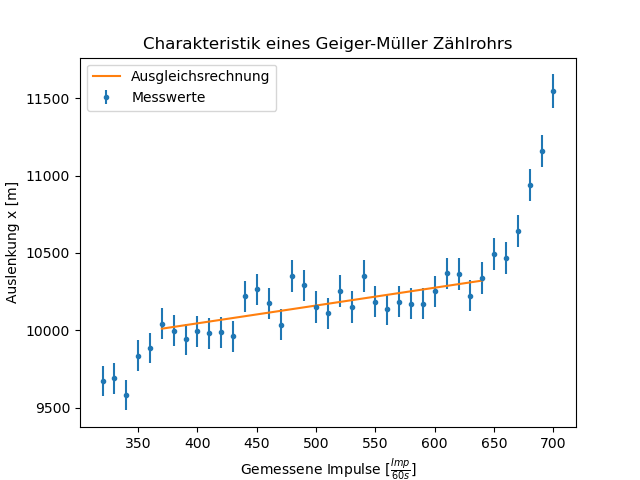
\includegraphics{7a.png}

\subsection{Länge des Plateau-Bereichs}

\noindent In diesem Diagramm ist ein Plateau zu erkennen.
Es erstreckt sich von einer Spannung von 370V bis zu einer Spannung von 640V.
Die Länge dieses Plateau-Bereichs beträgt also 270V.

\subsection{Plateau-Steigung}

Für die Plateau-Steigung wurde eine Ausgleichsrechnung mit der Python-Funktion "$curve_fit$" aus "$scipy.optimize$", im Plateau-Bereich, durchgeführt.
Dafür wurde eine Funktion der folgenden Form verwendet:

\begin{displaymath}
    y = mx + n
\end{displaymath}

\noindent Für die Parameter m und n ergibt sich:

\begin{center}
    \begin{tabular}{ll@{${}\pm{}$}l}
        \toprule
        Parameter & Wert & Unsicherheit\\
        \midrule
        m &    1.151888 & 0.223673 \\
        n &   9584.296388 & 114.390865 \\
        \bottomrule
        
    \end{tabular}
\end{center}

\noindent Dabei ist zu sagen, dass der Parameter m den Wert $\frac{1}{60Vs}$ und der Parameter n die Einheit $\frac{1}{60s}$ hat.

\noindent Die geforderte Plateau-Steigung ergibt sich durch folgende Gleichung:
\begin{align}
    PS &= \frac{m}{60} \;\;\;\;\;\;\;\;  \text{Umrechnung auf 1/V} \nonumber \\
    PS &= \frac{m}{60}  * 100\%  \nonumber 
\end{align}

\noindent Die Plateau-Steigung in $\frac{\%}{100V}$ hat den Wert:

\begin{displaymath}
    (1.9198 \pm 0.3728) \frac{\%}{100V}
\end{displaymath}

\section{Aufgabe 7b}

\section{Aufgabe 7c}

\noindent Die Totzeit des Zählrohrs lässt sich mit der Zwei-Quellen-Methode durch folgende Formel bestimmen:

\begin{displaymath}
    T = \frac{N_1+N_2-N_{1+2}}{2N_1N_2}
\end{displaymath}

\noindent Mit den Werten:

\begin{align}
    N_1 &= (96041 \pm 309.9048) \frac{1}{120s} = (800.3 \pm 2.6) \frac{1}{s} \nonumber \\
    N_{1+2} &= (158479 \pm 398.0942) \frac{1}{120s} = (1320.7 \pm 3.3) \frac{1}{s} \nonumber \\
    N_2 &= (76518 \pm 276.6189) \frac{1}{120s} = (637.6 \pm 2.3) \frac{1}{s} \nonumber
\end{align}

\noindent ergibt  sich die Totzeit zu $(115 \pm 4)\mu s$.

\section{Tabellen}
\begin{minipage}{\linewidth}
    \begin{table}[H]
        \centering
    
    \begin{tabular}{ll}
        \toprule
        Spannung [V] & Impulse [$Imp/60s$]\\
        \midrule
        320 &	9672   \\   
        330 &	9689   \\  
        340 &	9580   \\   
        350 &	9837   \\   
        360 &	9886   \\    
        370 &	10041  \\    
        380 &	9996   \\   
        390 &	9943   \\   
        400 &	9995   \\   
        410 &	9980   \\    
        420 &	9986   \\   
        430 &	9960   \\  
        440 &	10219  \\
        450 &	10264  \\
        460 &	10174  \\
        470 &	10035  \\
        480 &	10350  \\
        490 &	10290  \\
        500 &	10151  \\
        510 &	10110  \\
        520 &	10255  \\
        530 &	10151  \\
        540 &	10351  \\
        550 &	10184  \\
        560 &	10137  \\
        570 &	10186  \\
        580 &	10171  \\
        590 &	10171  \\
        600 &	10253  \\
        610 &	10368  \\
        620 &	10365  \\
        630 &	10224  \\
        640 &	10338  \\
        650 &	10493  \\
        660 &	10467  \\
        670 &	10640  \\
        680 &	10939  \\
        690 &	11159  \\
        700 &	11547  \\      
        \bottomrule
        
    \end{tabular}
    \captionof{table}{Gemessene Impulse bei verschiedenen Spannungen}
    \label{tab:7a}
    \end{table}
    \end{minipage}
\end{document}